\newpage
\section{Resultados}

\subsection{Atividade 1 – Circuitos Ressonantes}

Para o circuito ressonante da figura \ref{fig:05}, primeiramente calculamos 
a frequência de ressonância, como mostrado abaixo:

\[
  f_0 = \frac{1}{2 \pi \sqrt{LC}} = \frac{1}{2 \pi \sqrt{2.10^{-6} \times 
  22.10^{-9}}} = 758,54 \ [kHz].
\]

A frequência de ressonância medida foi muito próxima da frequência de 
ressonância calculada, tendo um valor de 758,57 kHz.
Para a frequência de ressonância analisada no gráfico, observamos uma tensão de 
pico correspondente a 903,84 mV.

\begin{figure}[H]
  \centering
  \caption{Sinal da função de transferência para um circuito ressonante 
  paralelo.}
  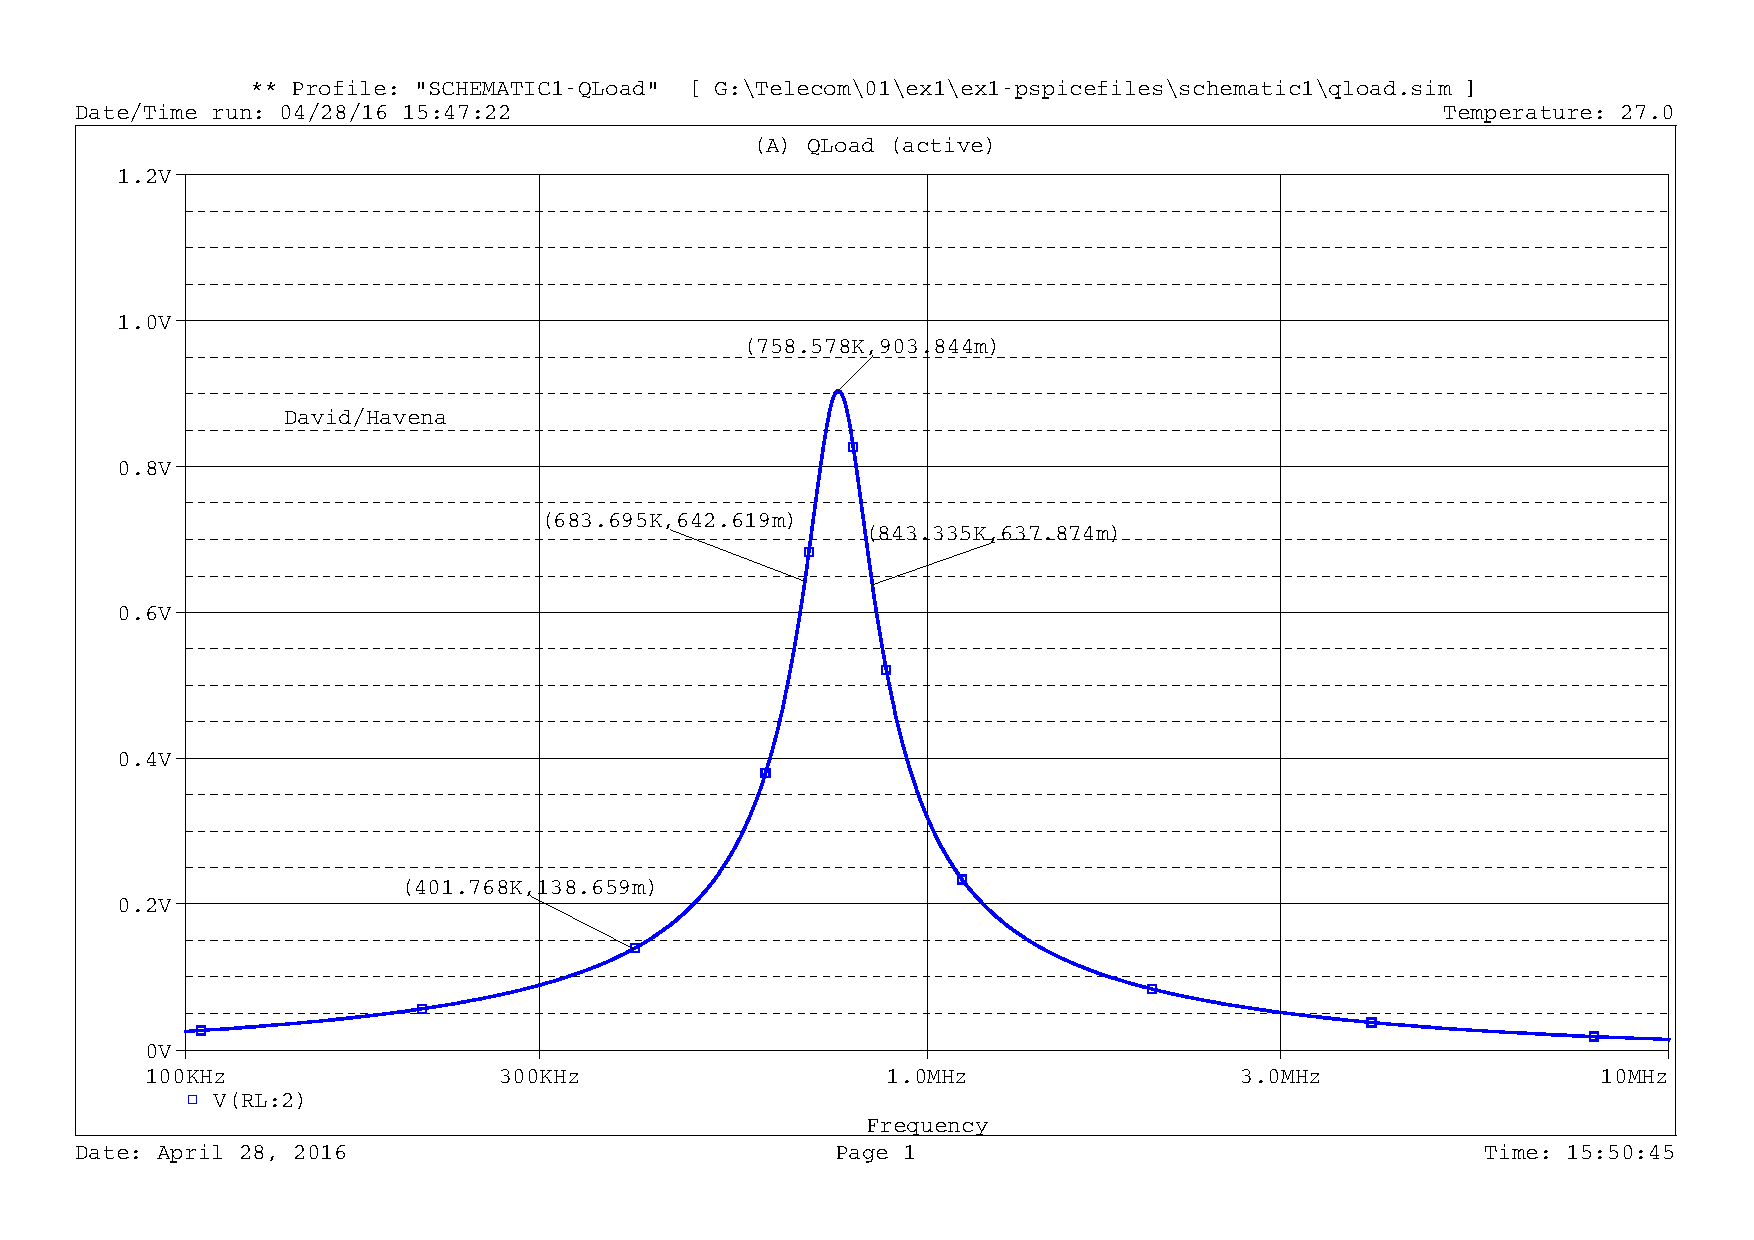
\includegraphics[scale=0.5]{05.pdf}
  
  \label{fig:05}
\end{figure}

A tensão de largura de banda foi calculada, utilizando-se a tensão de pico 
correspondente a frequência de ressonância, como mostrado abaixo:

\[
  V_{c} = \frac{V_p}{2} = \frac{903,84.10^{-3}}{2} = 639,1.10^{-3} \ [V]
\]

Com isso, encontraram-se no gráfico frequências de 0,995 MHz e 1,157 MHz.
A partir dessas frequências obtivemos também a largura de banda (BW) que é equivalente a 0,162 MHz.
Utilizou-se então a equação 2 para calcular o índice de mérito do circuito que resultou em 4,75.

\[
  Q_{Load} = \frac{f_c}{BW} = \frac{758,57.10^3}{162.10^3} = 4,68
\]

Para calcular o índice de mérito do circuito teoricamente, deve-se calcular a resistência equivalente. O calculo da resistência equivalente segue abaixo:

\[
  R_e = \frac{R_S R_L}{R_S + R_L} = \frac{470 \times 50}{470 + 50} = 45,19 \ [\Omega]
\]

Dividindo a resistência equivalente pela frequência angular de ressonância foi possível encontrar um índice de mérito muito próximo do valor obtido na prática.

\[
  Q_{Load} = \frac{R_e}{2\pi f_0L} = \frac{45,19}{2\pi  758,57.10^3 \ 2.10^{-6}}
\]

Em seguida, o fator de qualidade do indutor foi calculado, assumindo-se um valor para a resistência interna igual a 1,5 $\Omega$.

\[
  Q_{Load} = \frac{X_L}{r_s} = 6,49
\]

Por fim, o índice de rejeição para a frequência de 0,53*f0 foi calculada:

\[
  \frac{E_0}{E} = \sqrt{1 + Q^2 \left(\frac{f}{f_0} - \frac{f_0}{f}\right)^2}
\]

\[
  E = 145,69 \ [mV] = -16,73 \ [dB]
\]

\subsection{Atividade 2}

\subsubsection{Filtro Passa-Baixas (FPB)}
Para a segunda atividade, projetou-se um filtro passa-baixas RC passivo com os seguintes parâmetros: $f_c$ = 276 Hz e C = 150 nF.

\[
  R = \frac{1}{2 \pi F C} = 3,844 \ [k \Omega]
\]

Com o filtro projetado, obtivemos a resposta em frequência como mostra a figura \ref{fig:06}.

\begin{figure}[H]
  \centering
  \caption{Módulo da resposta em frequência.}
  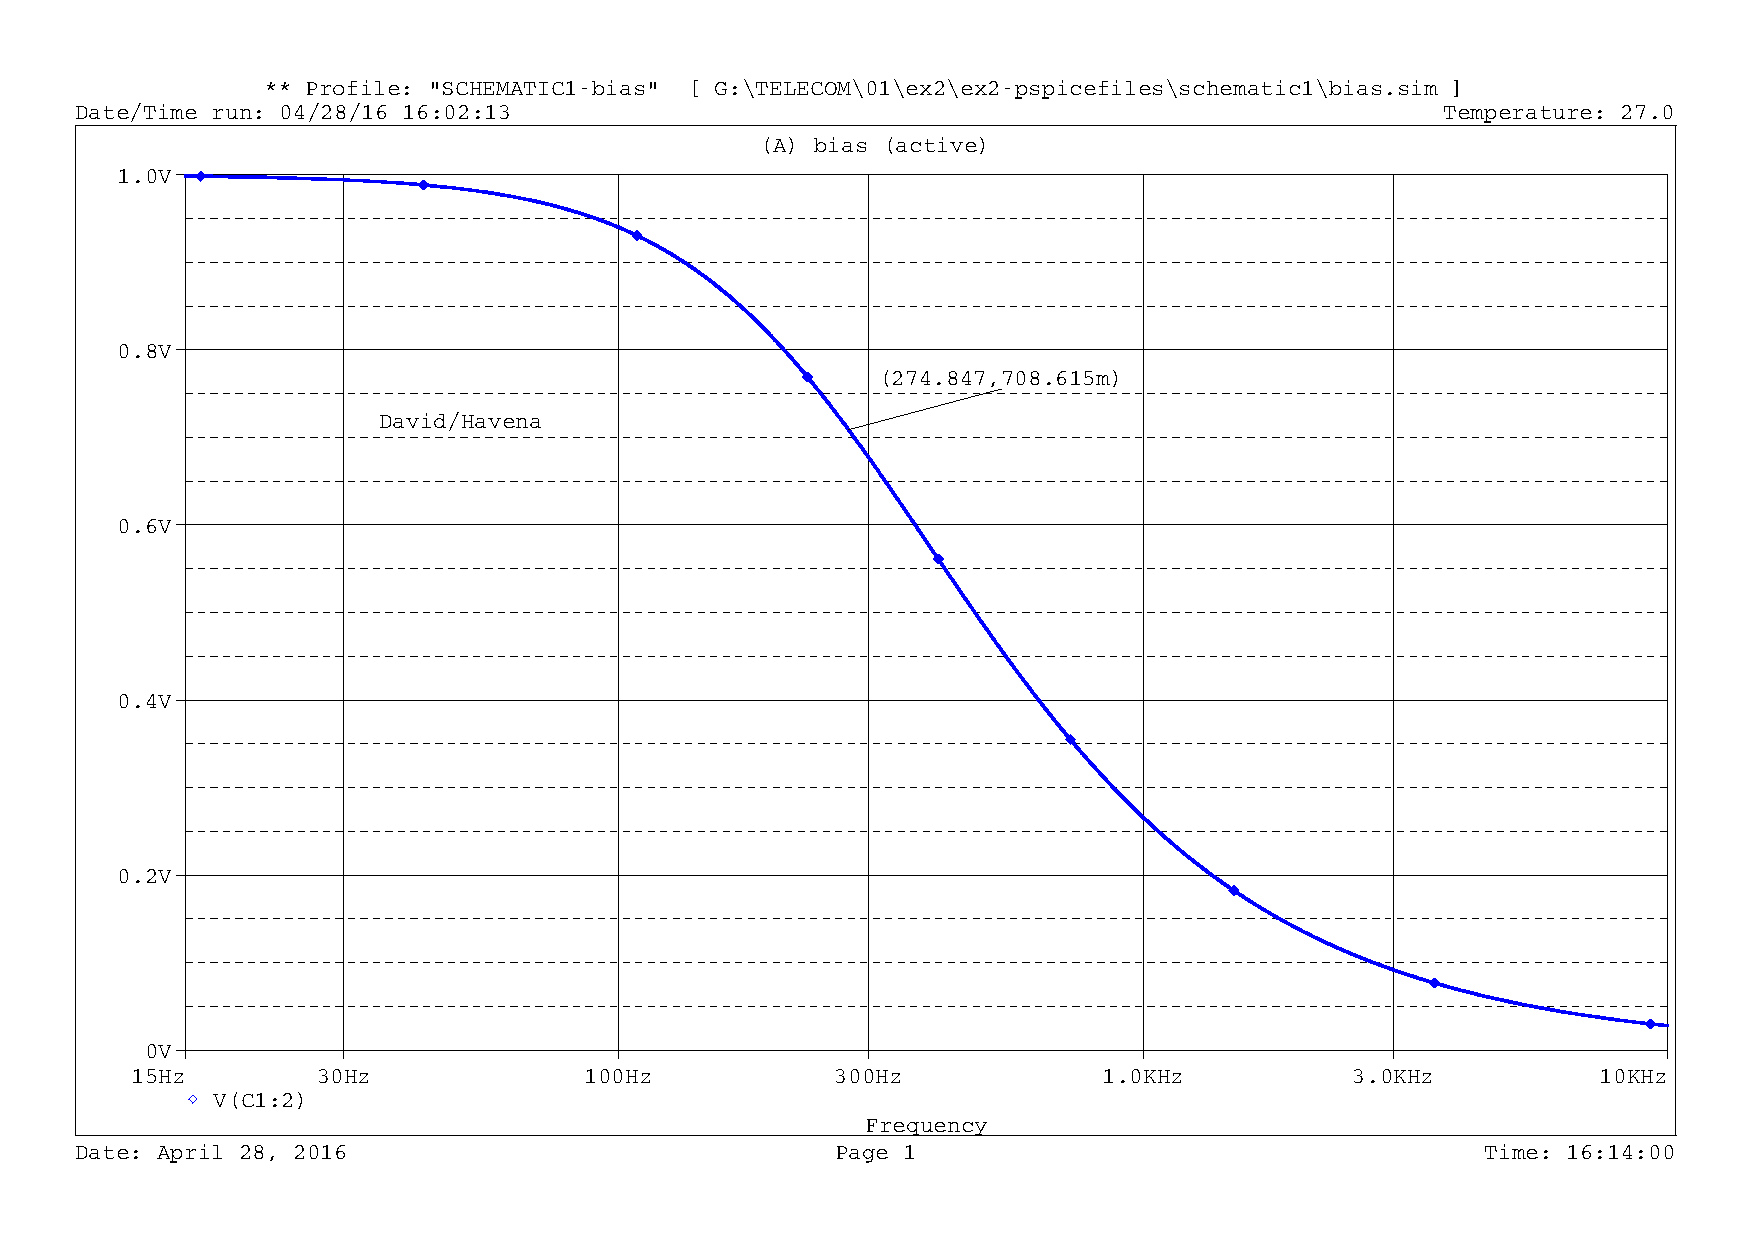
\includegraphics[scale=0.4]{06}
  
  \label{fig:06}
\end{figure}


A figura \ref{fig:07} mostra a fase da resposta em frequência.

\begin{figure}[H]
  \centering
  \caption{Fase da resposta em frequência.}
  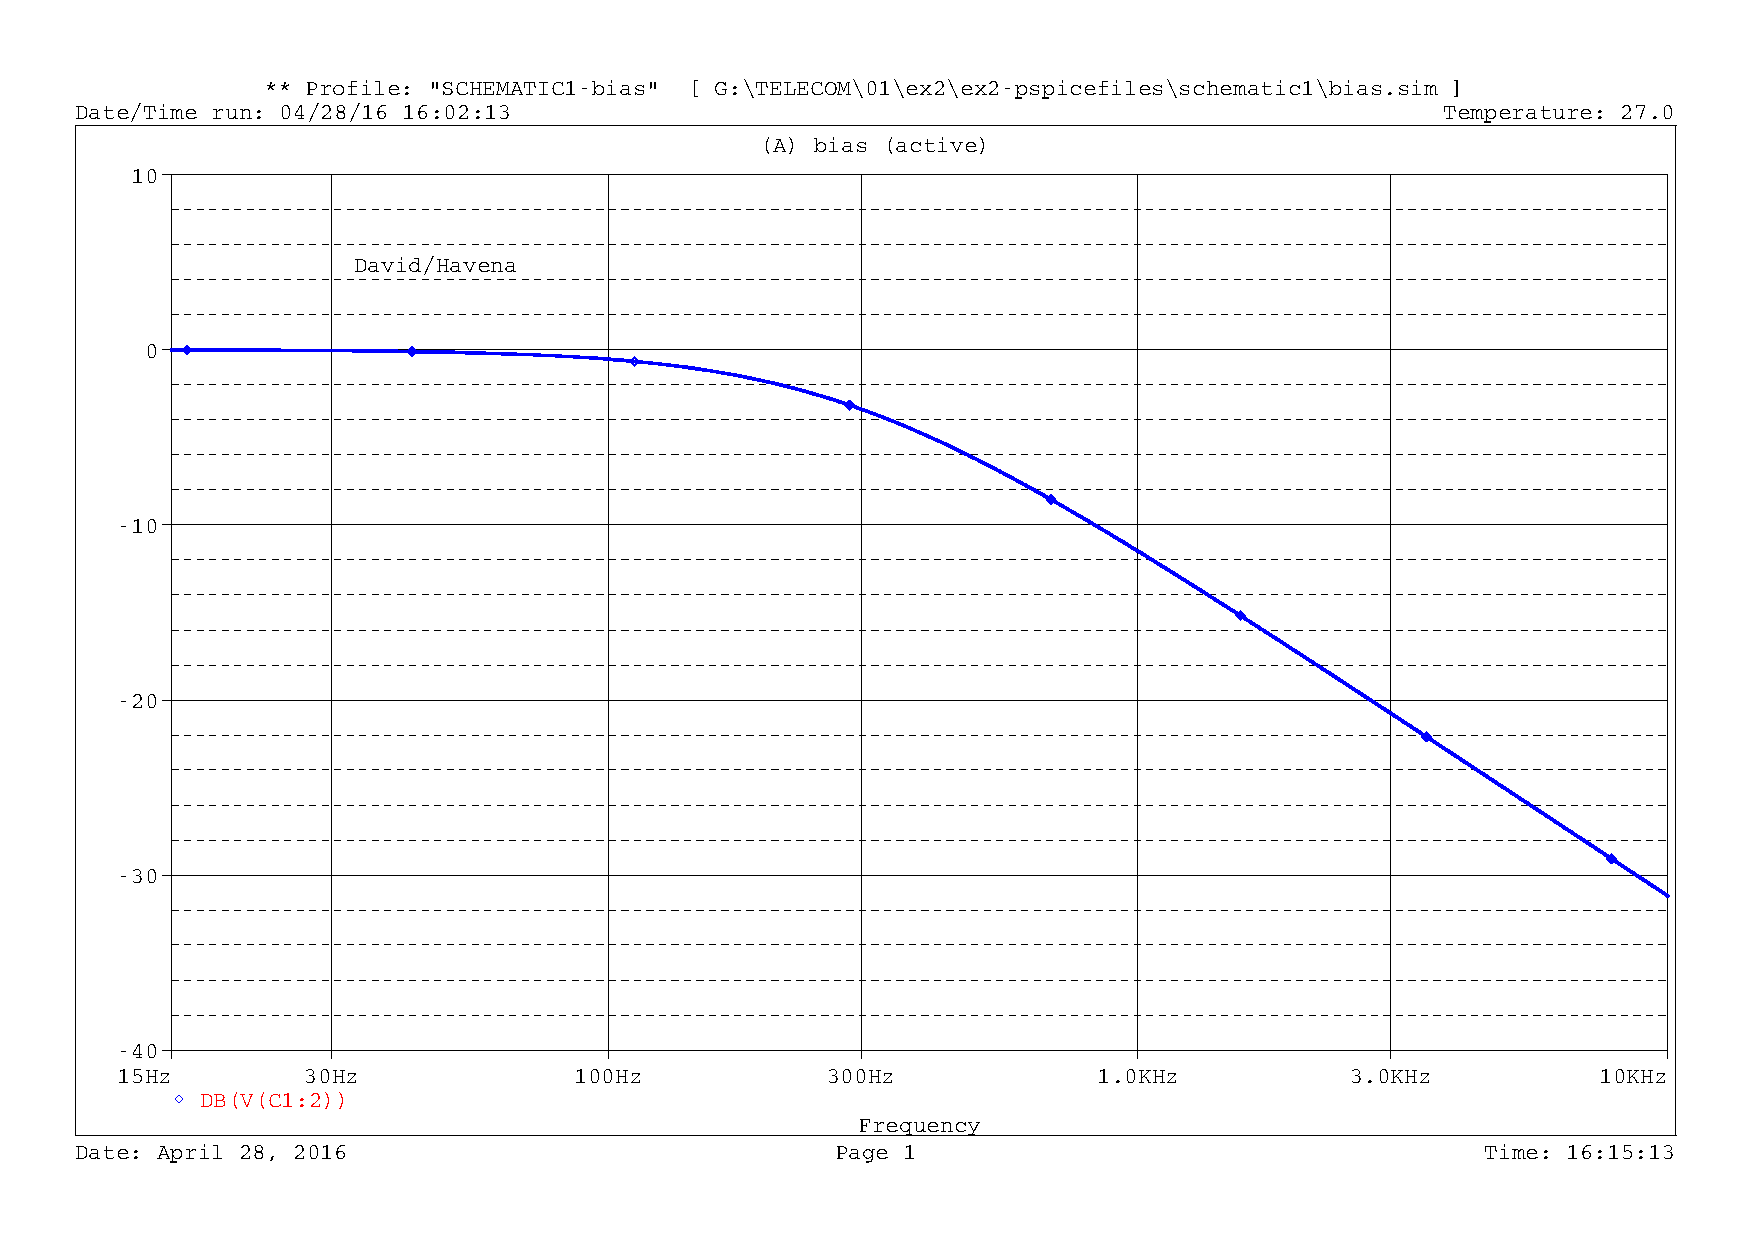
\includegraphics[scale=0.4]{07}
  
  \label{fig:07}
\end{figure}

Por fim, foi obtido o gráfico de Lissajous como mostra a figura \ref{fig:08}. A partir do gráfico obtivemos os pontos de cruzamento com o eixo positivo e negativo. Com esses pontos calculamos A e B e consequentemente a defasagem.

\[
  \Delta \Theta = sen^-1 \left(\frac{1}{1,4}\right) = 45 \ [graus]
\]
\begin{figure}[H]
  \centering
  \caption{Gráfico de Lissajous do Filtro Passa-Baixas Passivo.}
  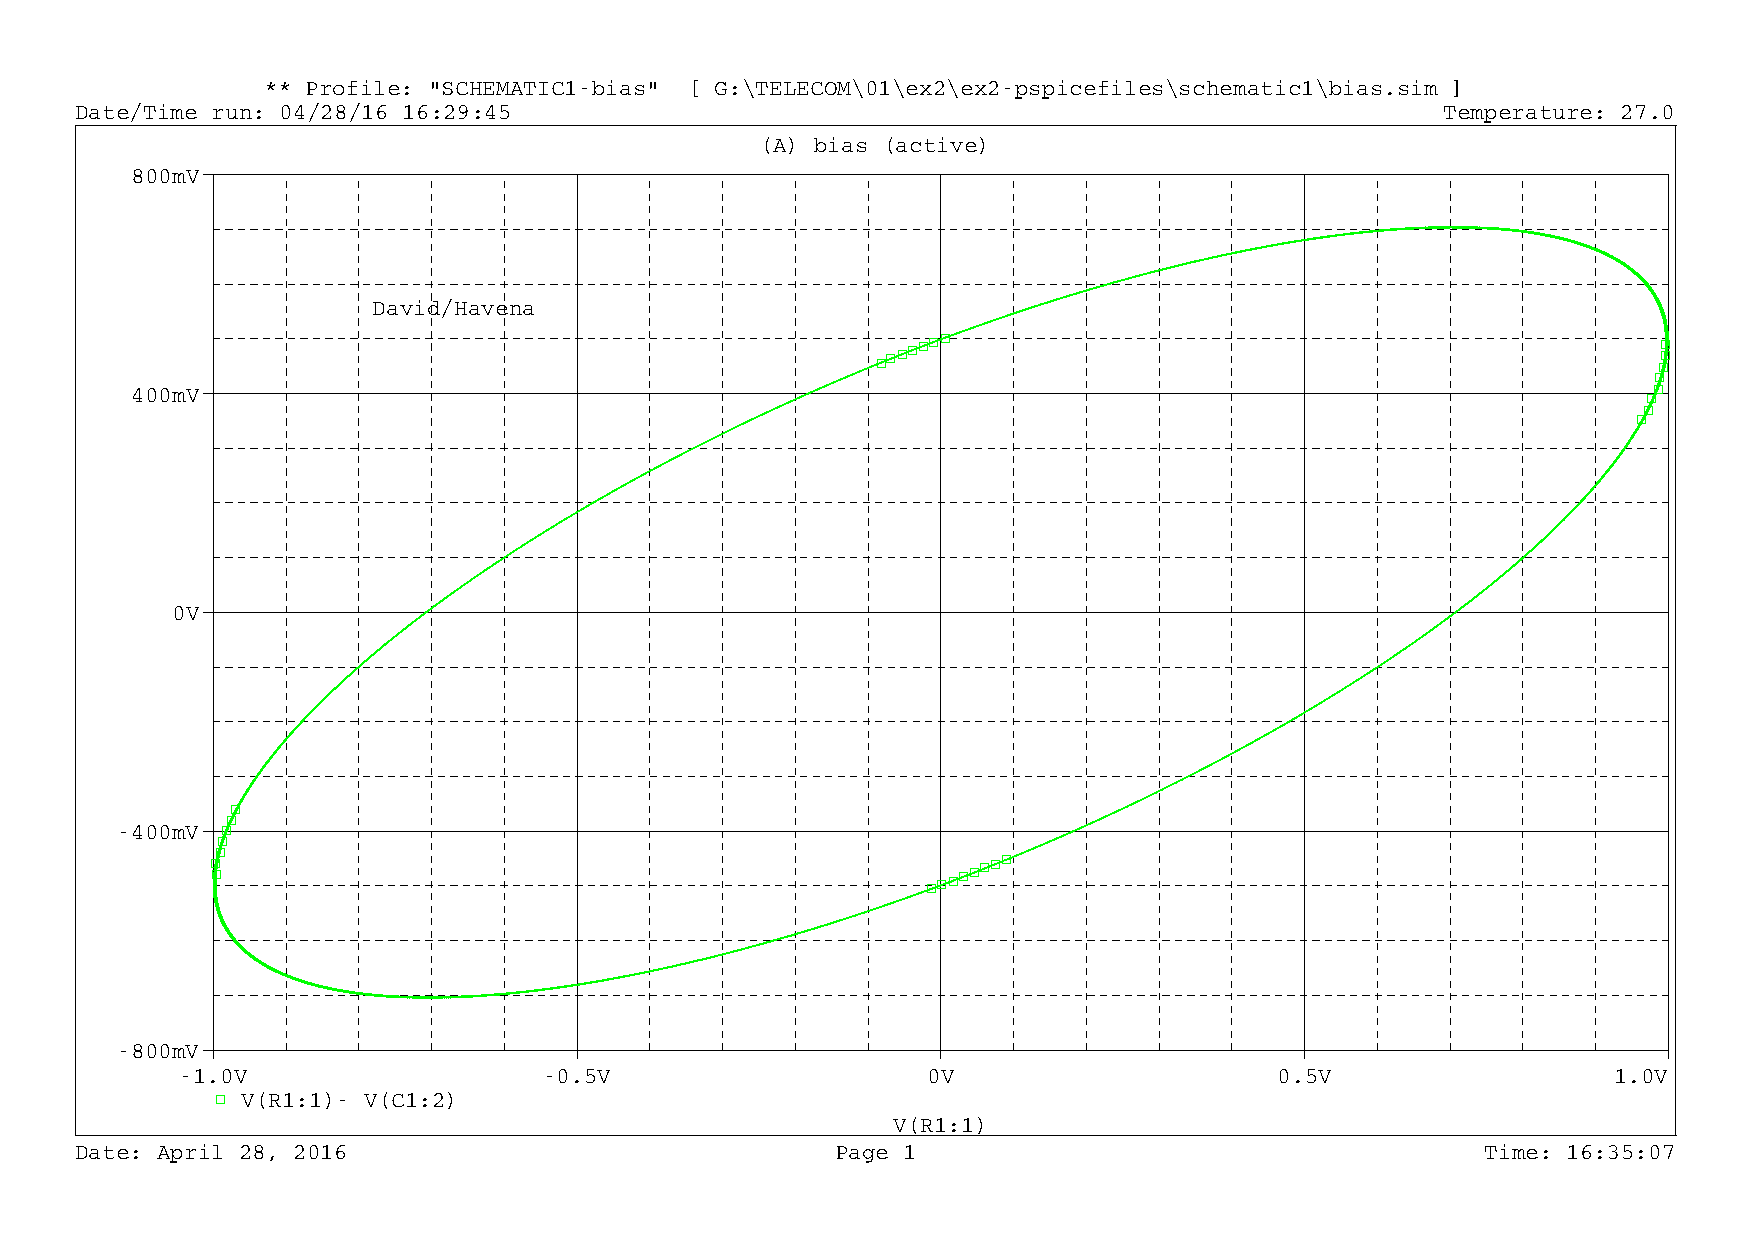
\includegraphics[scale=0.4]{08}
  
  \label{fig:08}
\end{figure}

\subsubsection{Filtro Passa-Altas (FPA)}

Nesta ultima prática projetou-se um filtro passa-altas RC passivo com os seguintes parâmetros: $f_c$ = 5,2 kHz e C = 150 nF.

\[
  R = \frac{1}{2 \pi F C} = 204,04 \ [ \Omega]
\]

Com o filtro projetado, obtivemos a resposta em frequência como mostra a figura \ref{fig:09}.

\begin{figure}[H]
  \centering
  \caption{Módulo da resposta em frequência.}
  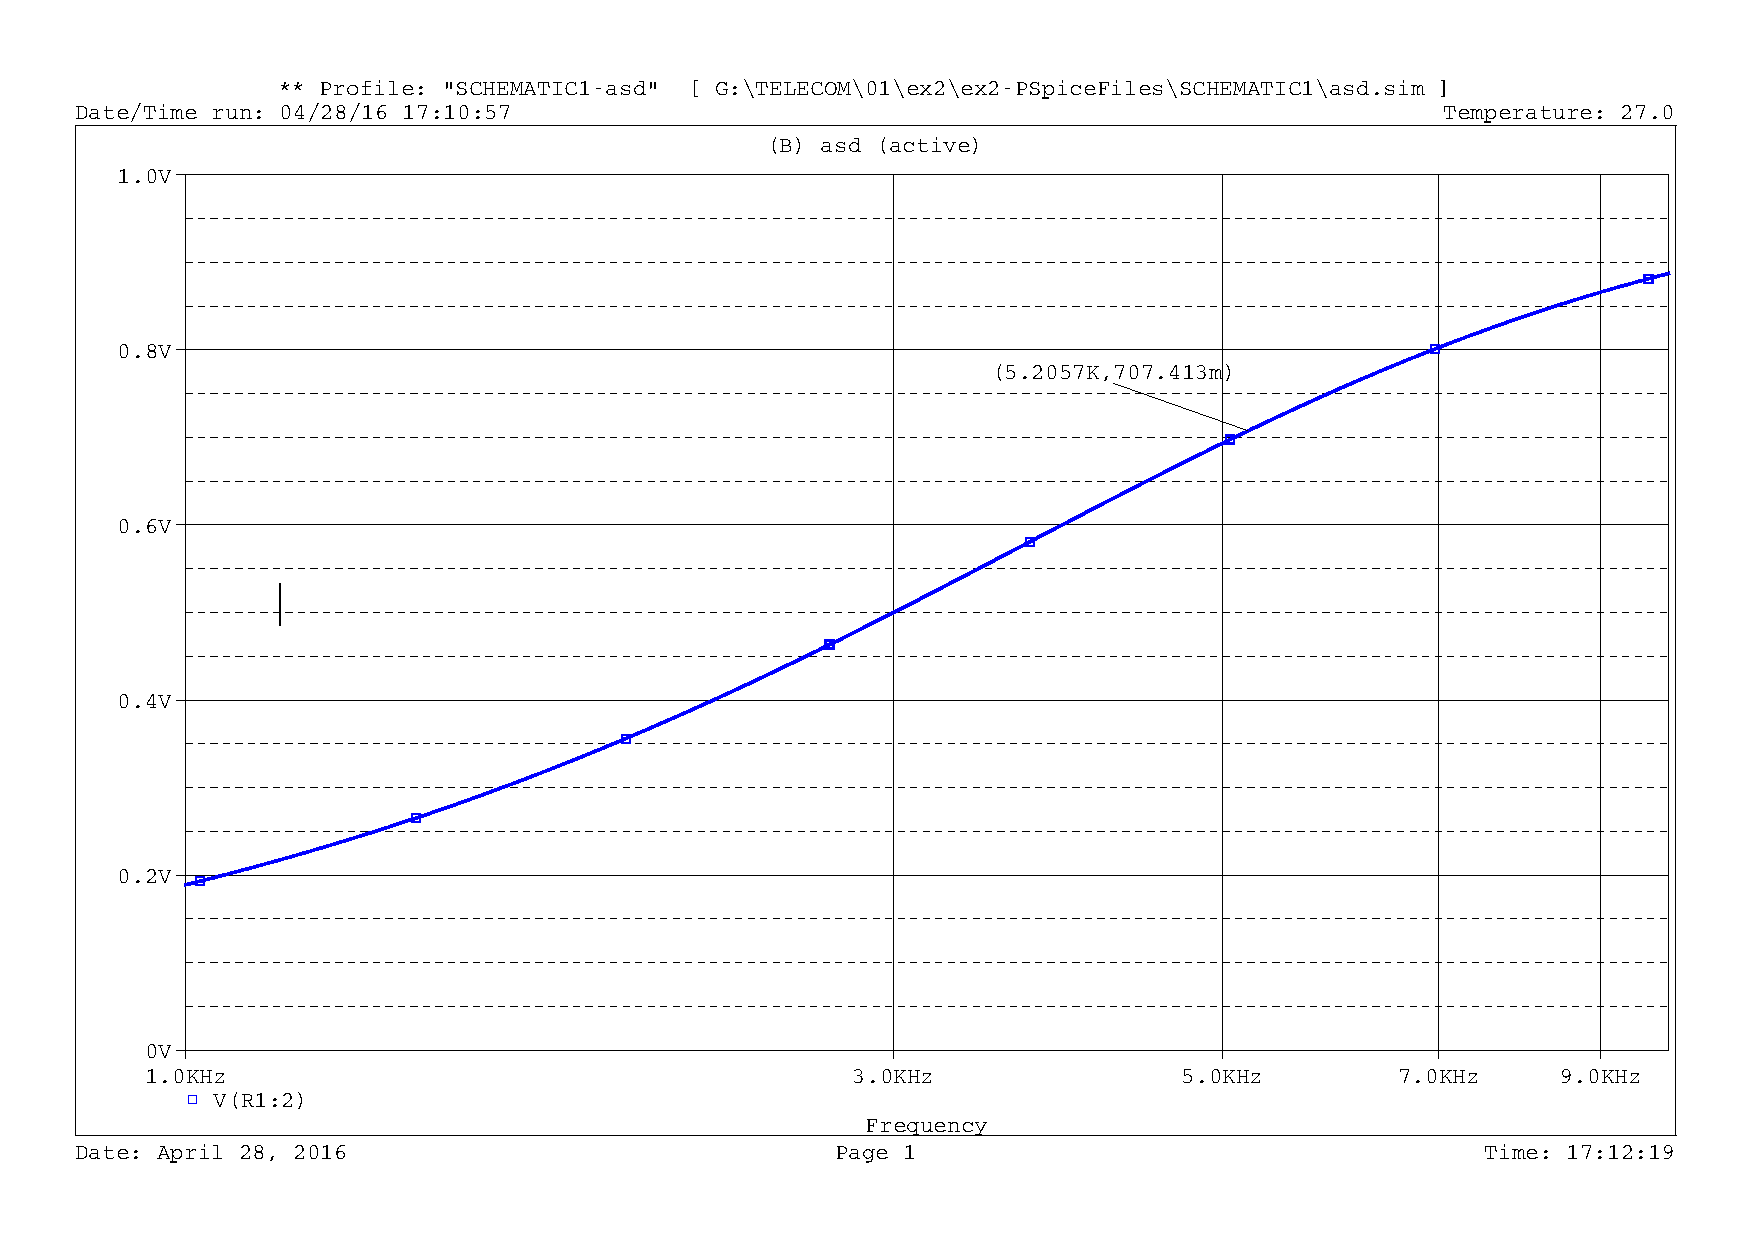
\includegraphics[scale=0.4]{09}
  
  \label{fig:09}
\end{figure}


A figura \ref{fig:10} mostra a fase da resposta em frequência.

\begin{figure}[H]
  \centering
  \caption{Fase da resposta em frequência.}
  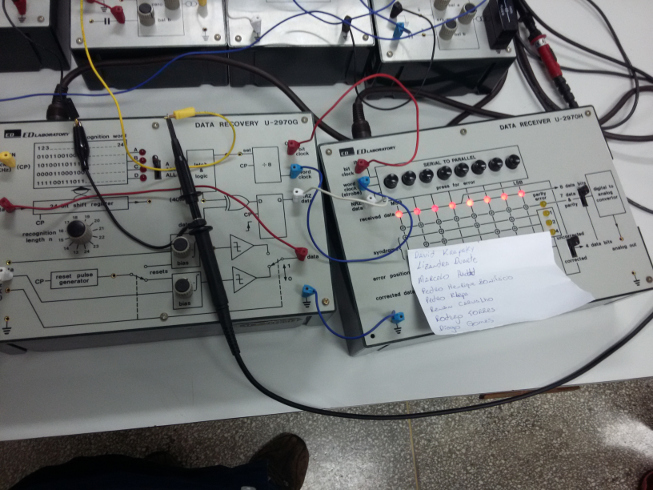
\includegraphics[scale=0.4]{10}
  
  \label{fig:10}
\end{figure}

Por fim, foi obtido o gráfico de Lissajous como mostra a figura \ref{fig:11}. A partir do gráfico obtivemos os pontos de cruzamento com o eixo positivo e negativo. Com esses pontos calculamos A e B e consequentemente a defasagem.

\[
\Delta \Theta = sen^-1 \left(\frac{1}{1,4}\right) = 45 \ [graus]
\]
\begin{figure}[H]
  \centering
  \caption{Gráfico de Lissajous do Filtro Passa-Baixas Passivo.}
  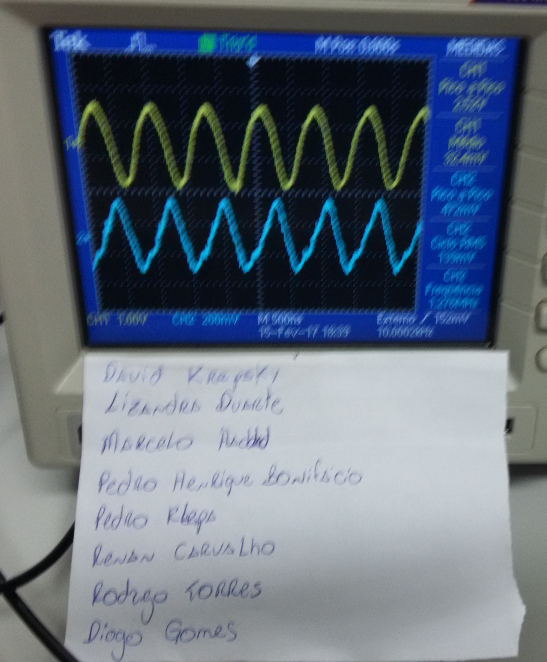
\includegraphics[scale=0.4]{11}
  
  \label{fig:11}
\end{figure}